%%%%%%%%%%%%%%%%%%%%%%%%%%%%%%%%%%%%%%%%%%%%%%%%%%%%%%%%%%%%%%%%%%% 
%                                                                 %
%                            CHAPTER ONE                          %
%                                                                 %
%%%%%%%%%%%%%%%%%%%%%%%%%%%%%%%%%%%%%%%%%%%%%%%%%%%%%%%%%%%%%%%%%%% 
 
\chapter{INTRODUCTION}
 
\section{Motivation}
At the turn of 2017/2018,  global warming has been unequivocally proved by scientific evidence~\cite{nasa_warm}. 
The surface temperature of Earth has risen by 2.0 degrees Fahrenheit since the late 19th century.  The ice sheets, glaciers and Arctic sea ice are retreating almost everywhere on Earth, at an accelerating speed. Extreme weathers like tornados, heatwaves, wildfires and droughts are increasing in frequency and intensity. There is no doubt that human activities, especially manmade emissions carbon dioxide (CO2) and other exhausts like nitrogen oxides, carbon monoxide, sulphur oxides are the major causes. 

Air transport is responsible for about $2\%$ of the manmade carbon dioxide (CO2) emissions~\cite{aviation_warm}. But because of the altitude the CO2 is released, together with the fact that other emissions like NOx and water vapor having a larger impact on the climate at higher altitudes, researchers suggest that aviation CO2 emissions should be multiplied by 1.9 times to incorporate the impact of altitude.   

With the airplane passengers growing at an average of $5\%$ each year, perhaps more at developing markets, the impact of aviation on the environment will only increase. It is estimated that approximately 27,000 new passenger aircrafts will be demanded between now and 2030.  The total contribution of aviation to human emissions in CO2 and other effects will rise to $5\%$ and a worst-case $15\%$. 

Advisory Council for Aeronautics Research in Europe (ACARE) is enforcing strict emission targets, to reduce CO2 emissions per passenger kilometer by $75\%$, NOx by $90\%$ and perceived noise by $65\%$ by 2050 relative to the year 2000~\cite{SKINNER2018933, euro_commi}. Reducing the impact on the environment is becoming the driving factor for future aircraft design~\cite{green_2006}. To do that, the aviation industry needs to continue working on reducing gas emissions by using light weight and smart materials, and optimizing current aircraft configurations. 

%technology, like exploring innovative aircraft shapes, improving current aircraft efficiency by minimizing drag for aerodynamic shape optimization, or minimizing mass for structural optimization, and upgrading operations to reduce noise and delays. 

\section{The Role of Numerical Optimization}
The ultimate goal of engineering is to make better decision-making models through optimization. Numerical optimization plays a key role in almost every aspect of engineering design.  

The aircraft design is a complicated system that involves aerodynamics, structures, propulsion, stability, mission and whole performance. The past two decades has seen growing interests in using optimization to explore unconventional aircraft configurations like the blended-wing body (BWB), the Box Wing, the UCAV (Unmanned Combat Air Vehicle). During the conceptual 
aircraft design stage, numerical optimization can reveal valuable insights about the design trade-offs and help engineers make detailed and informed decisions.  
     
The first aerodynamic optimization was done in \cite{hicks:1974} by using finite-difference approximations to calculate the gradients. The cost of computing the gradients using finite-difference methods increase drastically as the design dimension increases. The adjoint methods greatly propelled the advancement of research in aerodynamic shape optimization field. Adjoint methods address the dimensionality issue of finite-differences with a cost independent of the number of design variables. \cite{pironneau:1974} developed the adjoint method for Stokes equations and the incompressible Euler equations, and used the adjoints to optimize airfoil profiles. \cite{reuther:1996} used an adjoint algorithm based on Euler to optimize a complete aircraft configurations.  \cite{jameson:1988} derived the adjoint equations for inviscid compressible Navier-Stokes equations, making it possible to do transonic aerodynamic optimizations.  The discrete adjoint method is more preferred in aerospace optimization as the sensitivities are exact to the discretized objective function~\cite{frank:1992}. \cite{Mader06adjoint:an} derived a discrete adjoint method for Euler equations using automatic differentiation. \cite{Lyu2013b} extended the previous adjoint implementation to 
Reynolds-averaged Navier-Stokes (RANS) equations and effectively applied it to high-fidelity optimization. \cite{hicken:aiaa2010} developed similar methods for non-planar wings high-fidelity aerodynamic optimization. 


%The ever-growing capacity of computers are empowering numerical analysts to do simulations on ever-larger physics systems governed by Partial-Differential-Equations(PDEs). Accordingly, PDE-constrained optimization problems pose greater challenges as the optimization systems are larger and more complicated, especially when many state-based constraints are present. Current matrix-based optimization algorithms are defied for such problems due to memory requirements and computing cost. 


\section{PDE-constrained Optimization Framework}
The thesis is interested in solving engineering design optimization problems that are governed by Partial-Differential-Equations (PDEs). Such PDE-constrained optimization problems arise in many engineering applications including aerodynamic shape optimization \cite{lambe:2014,lyu2014aerodynamic, Zhang567303}, structural optimization \cite{DBLP:DeckelnickHJ17, lambe:2014, kennedy14}, and thermodynamic optimization \cite{chen1999finite,bejan2000thermodynamic,bejan2012thermodynamic}.  %


\begin{figure}[H]
\centering
\subfloat[Aero-Structure Optimization~\cite{as_opt}]{
  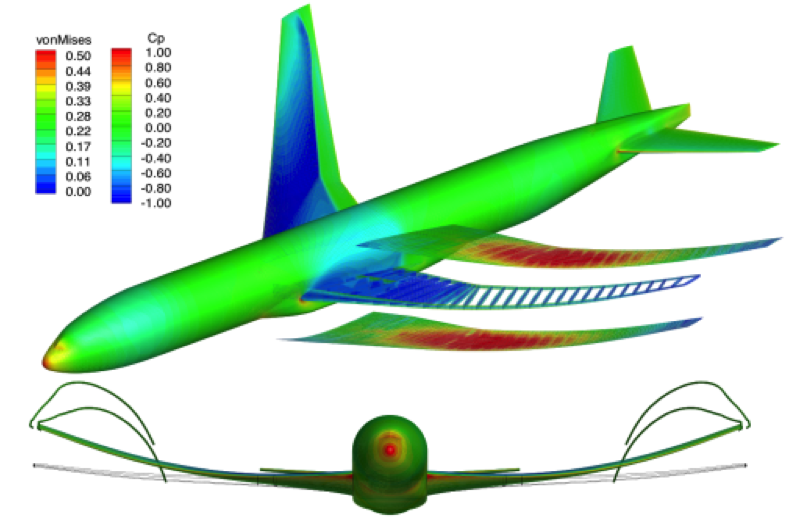
\includegraphics[clip,width=0.5\columnwidth]{./figs/chap1_intro/1_as.png}\label{fig:A}  %
}
\subfloat[Topology Optimization~\cite{topo_opt}]{ %
  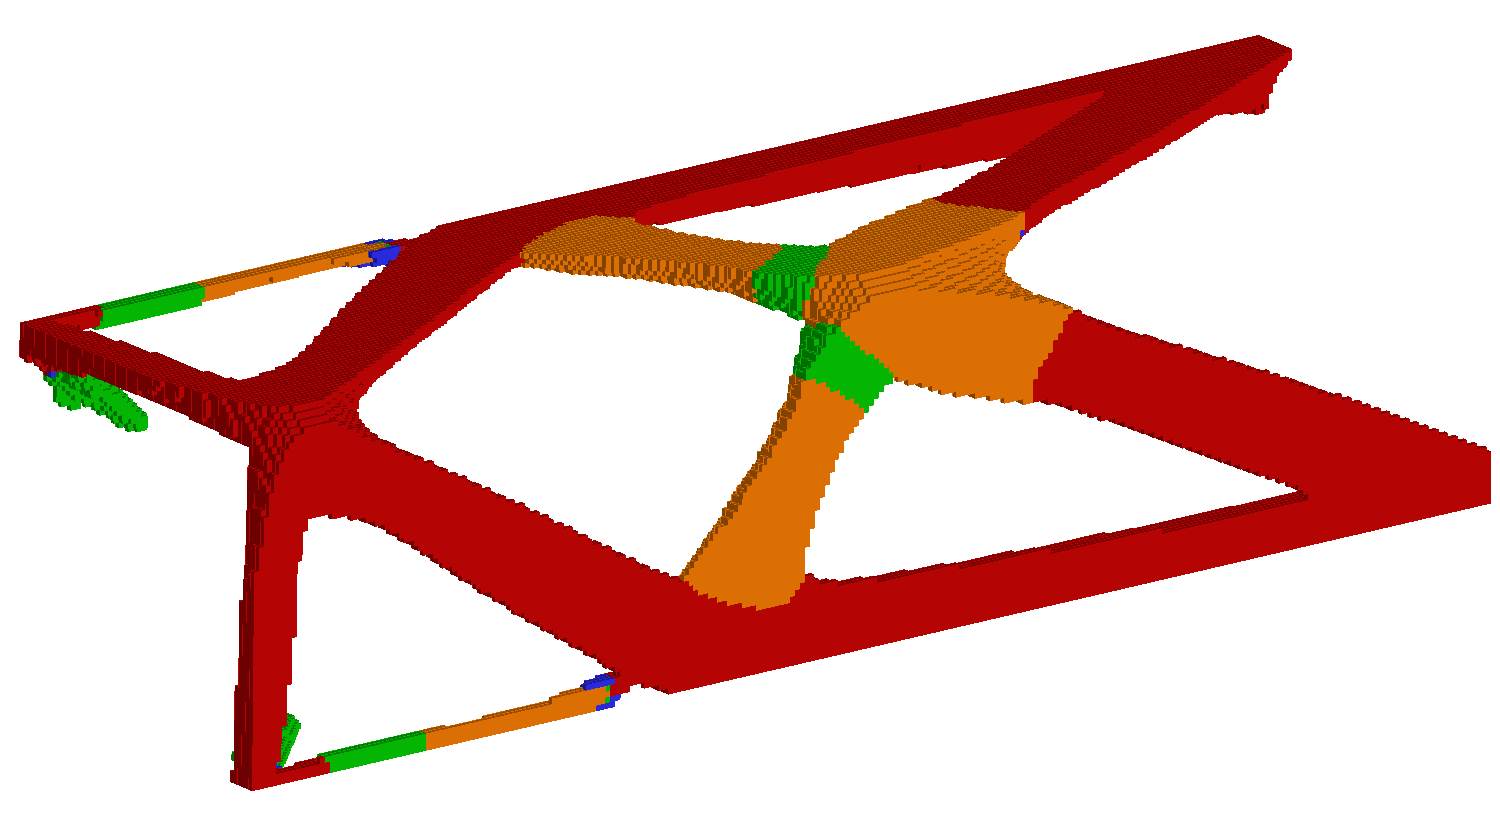
\includegraphics[clip,width=0.5\columnwidth]{./figs/chap1_intro/1_topo.png}\label{fig:B}
}
\caption{Large-Scale PDE-constrained Optimization}
\label{fig:1_mot}
\end{figure}

In such applications, an optimization library is coupled with a PDE solver. The simulation problem solves the PDEs for state variables, e.g. the pressure distribution along the surface mesh node points on the wing in Figure~\ref{fig:A}, the displacement distribution among the solid mesh node points in Figure~\ref{fig:B}, at certain design variables. The performance of the physics system is evaluated in the form of objective function bounded by certain constraints, while the objective and the constraints depend on both the state variables and the design variables. The optimizer will choose a design point, inquire the PDE solver for state variables, and compute the functional values and the gradients of the objective and constraints at that point. The optimizer will process all the information and yield a better design point using mathematical algorithms. The process is repeated until certain criteria is met for optimality.  

The optimization framework is simple, and has been used successfully in many application fields. The difficulty in PDE-constrained optimization is that the PDE solution (or state equation), which itself is a complicated topic to which intensive effort has been devoted, is a subproblem of the optimization problem. During the optimization process, the optimizer will query the PDE solver many times for the state variables and gradients at different design points; in addition to that, the optimizer need to compute and store the gradients of the constraints and objective in order to determine the next design point. In large-scale engineering, the PDE solve and gradient evaluation can be very expensive even with the advancement in modern computer power. Moreover, storage of the necessary matrices can impose a heavy burden on computational resources.    

General-purpose optimization algorithms are unsuitable for large-scale PDE-constrained optimization problems, because their matrix-based approaches require the computation and storage of the total constraint Jacobians, which in turn would result in poor scalability performance with ever-increasing size of problems. In addition, the commonly used limited-memory quasi-Newton methods in general-purpose algorithms usually brings linear asymptotic convergence rates, which is not ideal for large-scale optimization problems. 

This thesis intends to address these challenges by proposing a scalable optimization algorithm specially for large-scale PDE-constrained design problems. 

\section{Optimization Algorithms}
Many optimization packages are available for applications of different types. Considering the expensive cost of PDE solutions in PDE-constrained optimization problems, it is crucial to choose an efficient optimization algorithm that uses less number of function evaluations. Besides, the optimization algorithm must be able to handle nonlinear objectives and constraints. Gradient-free optimization algorithms like the genetic algorithm are not suitable here because they demands large amounts of function calls, despite the fact that they can locate global minimums. Gradient-based algorithms are used extensively in PDE constrained optimizations as they can handle hundreds of design variables by using the adjoint method to compute the gradients, with less number of function evaluations.  \cite{2015lyu_crm} and \cite{kenway:2014} use SNOPT (Sparse Nonlinear OPTimizer) \cite{gill:2002} through the Python interface pyOpt~\cite{Perez:2011:A} for the investigations of the aerodynamic and aerostructural optimization on the Common Research Model based on RANS, using analytically derived adjoint gradients. Because there are only three aerodynamic objective and constraints, drag, lift, pitch moment coefficients, they use the adjoint methods to assemble the total gradients to SNOPT. Other general purpose optimization algorithms can also work for aerodynamic design problems, IPOPT~\cite{Lyu2014f}, Knitro~\cite{Rumpfkeil2009OptimizationbasedMA}, a sequential quadratic programming method~\cite{Ning09multidisciplinaryconsiderations}. But they all compute the total gradients by using the adjoint methods and feed that to the optimization algorithm. 

For PDE-constrained optimization problems, when there are many state-based constraints, assembling the total constraint Jacobian is very expensive as it demands an adjoint solve for each state-based constraints. Besides, general optimization algorithm store the constraint Jacobians at each design point, which puts a heavy memory load on the computer. Therefore, most general optimization algorithms possess poor scaling qualities.  

For these reasons, optimization researchers in different PDE fields have been developing in-house algorithms for their own use. For detailed formulations, see chapter~\ref{sec:pde_mot}. Newton-based full-space methods possess good scaling, but is complicated to implement as it requires intrusion to the PDE solver. Currently there is no general purpose optimization libraries exist for full-space methods.  In addition, other numerical difficulties exist for full-space methods as pointed out in chapter~\ref{sec:pde_mot}. In comparison, reduced-space methods possess modularity that can make good use of prevalent PDE solvers. \cite{rumpfkeil:2010b} uses reduced-space Newton algorithm in KNitro to perform steady and unsteady aerodynamic shape optimization, with less computational cost compared with a quasi-Newton method; but the reduced Hessian is computed explicitly. In this work, we present a general reduced-space Newton-Krylov optimization algorithm, which is part of the matrix-free optimization package Kona~\cite{dener:scitech2016}, that makes use of the PDE solvers for different problems, and shares algorithmic scaling property as it approximates Hessian vector products through second adjoint solves. 

%Conventionally, solving general constrained optimization problems without PDE constraints involves forming the Lagrangian, and finding the minimization point of the Lagrangian, which is equivalent to solving the first-order optimality conditions or the KKT conditions. Prevalent sequential quadratic programming methods or newton-type methods for solving a system of equations would further break it down to solving a series of systems of linearized equations, also called the Karush-Kuhn-Tucker (KKT) system. The KKT matrix contains the Hessian of the Lagrangian, which is often approximated using quasi-Newton method, and the total constraint Jacobians, which is straightforward to compute using automatic differentiation or complex step methods. Conventional matrix-based optimization algorithms would use direct factorization methods to solve the KKT system.    


\section{Preconditioners for Optimization}
Using Krylov methods to solve the linear systems saves the effort of computing and storing the constraint Jacobian and Lagrangian Hessian, but the convergence rate of Krylov solvers depend on the distribution of eigenvalues of the system matrix. If the eigenvalues are clustered in a small radius, the convergence rate is better. Poor convergence happens when the ratio of the largest to the smallest absolute eigenvalue is large, ($10^5$ to $10^9$). 

In the context of PDE-constrained optimization problem, there are two sources of ill-condition. The first one resides in PDE solvers. When the discretization is refined, the eigenvalues of the PDE system matrix goes towards zero, or to say the PDE problem is ill-posed. The second source of ill-condition often arises from optimization algorithms like the interior-point method family, where slack variables are used to measure the activeness of the inequality constraints. When some of the inequality constraints get close to the boundary, the corresponding slack variables get near to zero, and certain entries on the diagonal of the KKT matrix will go unbounded. The second type of ill-condition is the target in this thesis, as the first type are usually covered as part of the PDE solver.     

In presence of ill-condition, a nonsingular matrix, the preconditioner, could do similarity transformation to the linear system, resulting in a better conditioned system with the same solutions.   

Several popular preconditioners exist for general optimization problems without PDE constraints, like incomplete factorizations~\cite{saad:2003}, which involve direct operations to the entries of the matrix,
or the null space approach, which involves computing and working with the null space of constraint Jacobians to find the step updates. Those preconditioners would not work well for interior-point methods type optimization problems, as the diagonal entries could go either zero or infinity for inequality constraints. Especially, for matrix-free PDE constrained optimization problems, the Hessian or constraint Jacobian do not exists in explicit form, so it is not possible to use direct methods.  

Inspired by domain-decomposed Schur preconditioners used in PDE solvers~\cite{keyes_domain} ,  where approximate subdomain solutions of the mesh field is used as preconditioners for the iterative solver of the PDE, \cite{DBLP:journals/siamsc/BirosG05} uses approximate state and adjoint solutions in the Schur of the KKT system as the preconditioner for the Krylov solver in each Newton step for the optimization problem. \cite{pc_kkt_control} presented a similar KKT matrix preconditioner for  optimization in distributed control problem using an interior-point method, it also used the block structure of the KKT matrix to decompose it, then used existing preconditioners for the PDE solvers to approximately solve the preconditioning system. However, the preconditioner is not ideal as the preconditioned system has both positive and negative eigenvalues. \cite{doi:10.1137/15M104075X} constructed a preconditioner for full-space Lagrange-Newton method for multi-field problems. The preconditioner removes the field variables that are causing nonlinearity of the system, resulting in a well-balanced Newton system. The preconditioner proposed in this thesis is similar to  \cite{pc_kkt_control}. 

%The kernel of reduced-space Newton-Krylov methods for PDE-constrained optimization solves a series of linear systems, which are saddle point systems, but much smaller than the saddle-point system raised in full-space methods.  Because the solution to the optimization problem \eqref{eq:opt00x} is a saddle point for the Lagrangian \eqref{eq:lag} in that the optimal design point minimizes the Lagrangian, while the optimal multipliers maximizes the Lagrangian ~\cite{benzi2005numerical}.  

\section{Thesis Objectives and Outline}

%The objective of this thesis is to develop an efficient inexact-Newton algorithm that is
%suitable for reduced-space PDE-constrained optimization problems of the
%form~\eqref{eq:gen1}.  This goal faces two significant challenges, which
%we seek to address in this work.
The thesis wants to overcome the challenges listed below, and doing so represents 
two separate objectives. 

\begin{description}
\item[Nonconvexity:] The system $F(q) =0$ does not distinguish between different
  types of stationary points, so a basic Newton's method may converge to local
  maximizers or saddle points.  Conventional optimization algorithms often
  project onto the null-space of the (active) constraint Jacobian to detect
  directions of negative curvature and avoid undesirable stationary points, but
  the null-space is not explicitly available for matrix-free inexact-Newton
  methods.
\item[Preconditioning:] The number of iterations necessary to satisfy the
  inexact Newton condition \eqref{eq:inexact_Newton} using, for example, a
  Krylov method is closely related to the condition number of the system.
  Unfortunately, it is well known that the primal-dual, or KKT, matrix $\nabla_q
  F$ is indefinite and highly ill-conditioned.  A preconditioner is needed that
  is inexpensive to form, factor, and store.  A general-purpose, inexpensive
  preconditioner is especially difficult to find in the reduced-space context,
  since approximations to $\nabla_q F$ are not readily available as they are in
  the full-space.
\end{description}

The approach to addressing globalization is to introduce a homotopy map that
implicitly defines a solution curve that connects the solution to an easy
problem to the solution of the desired problem.  We then use a
predictor-corrector algorithm to follow the curve from the easy to the desired
solution.  A related globalization is used in \cite{Perez2009homotopy} in the
context of a trust-region managed sequential approximate optimization.  To
address the conditioning of the KKT matrix, we propose a low-rank approximation
of the Schur complement that is constructed by applying a few iterations of the
Lanczos method with approximate adjoints.

The following contents are organized as follows: 
\begin{itemize}
\item Chapter 2 reviews homotopy-based globalization and the homotopy map adopted in this work. Then it describes the predictor-corrector path-following algorithm that traces the homotopy zero curve. 

\item Chapter 3 begins by reviewing Krylov iterative methods, but the focus is the proposed matrix-free preconditioner, firstly for solving inequality constrained problems, then for solving problems with both equality and inequality constraints. 
  
\item Chapter 4 begins with briefly introducing the optimization environment Kona, a state-of-the-art optimization algorithm SNOPT against which the performance of the new method is compared, and the parameter settings for the new method.  Then the optimization algorithm and preconditioners are tested on two analytical problems: 1) An indefinite problem to examine the algorithm's ability to bypass local maximum points. 2) A constructed quadratic problem with linear inequality constraints to investigate the scalability performance of the algorithm and effectiveness of the inequality-only preconditioner. 

\item Chapter 5 tests the Homotopy RSNK method, the inequality-only and mixed equality and inequality preconditioners on a subset of the CUTEr test problems. This Chapter briefly introduces CUTEr problems, the CUTEr problem classification and the Kona-CUTEr interface. Then it presents a table of numerical examples results using the new method and preconditioner, SNOPT.   
  
\item Chapter 6 applies the algorithm and preconditioner on a mass minimization stress-constrained structural problem. The results and the convergence history of the algorithm are compared with that of SNOPT.
  
\item Chapter 7 the new algorithm and preconditioner is applied on an aerodynamic shape optimization problem. The results and the convergence history of the algorithm are compared with that of SNOPT.

\item Chapter 8 provides conclusions and some suggestions for future works. 
\end{itemize}


% a popular large-scale matrix-based active -set augmented-Lagrangian optimization method SNOPT.  

%\begin{equation}\label{eq:saddle}
%\mathcal{A} = \begin{bmatrix}
%A & B \\
%C & D
%\end{bmatrix}
%\end{equation}
%One type of Schur complement can be obtained by performing the following LDU decomposition 
%\begin{equation}\label{eq:saddle:ldu}
%\mathcal{A} = \begin{bmatrix}
%A & B \\
%C & D
%\end{bmatrix} = 
%\begin{bmatrix}
%I_p & BD^{-1} \\
%0 & I_q
%\end{bmatrix}
%\begin{bmatrix}
%A-BD^{-1}C  & 0 \\
%0  & D 
%\end{bmatrix}
%\begin{bmatrix}
%I_p  & 0 \\
%D^{-1}C  & I_q 
%\end{bmatrix}
%\end{equation}

% which is indefinite, poor spectral properties (ill-conditioned) 
% Direct solvers, however, are still the preferred method in optimization and other areas. Furthermore, direct methods are often used in the solution of subproblems, for example as part of a preconditioner solve.
%The preconditioners developed here are tailored for PDE-constrained optimization problem. 
% matrix-vector products with A can be performed efficiently
% approximate its action on a vector with (nearly) linear complexity,
% the convergence of the iterates to the optimal solution of problem
% gain efficient, save on storage
%words from the paper ~\cite{benzi2005numerical} Benzi block preconditioners, 
% As the iterates approaches the solution,  the entries in A tend to zero, or infinity, KKT matrix ill-conditioned
% the norm of the inverse Schur complement goes to infinity

% Schur complement reduction 
% null space methods, the null space of the constraint Jacobian, the column of Z span the null space of constraint Jacobian
% popular in optimization, projection of the problem onto the constraint set; 

 
%%% Local Variables: 
%%% mode: latex
%%% TeX-master: t
%%% End: 

%The formula \eqref{eq:kkt0} takes the same form as the classical interior point method in Chapter 19 in Nocedal's book \cite{Nocedal2006NO}, which will be reviewed below. 

%\section{Review on Interior Point Method  }
%The difficulty in extending the Newton Krylov methods to handle inequality constraints, to solve \eqref{eq:opt00x} lies in the nonlinear complementarity condition: for each inequality constraint, either the slack or Lagrangian multiplier is strictly zero if we assume strict complementarity is satisfied at the solution. The slack has to be non-negative to guarantee feasibility of the inequality constraints, and the multipliers has to be non-positive in respect to the property of a local minimization point following the formula convention. For inequality constraints that are active at the solution, slack variable is zero and the multiplier is negative, while for inactive inequality constraints, slack variable is positive and the multiplier is negative. Therefore, the complementarity condition, in combined with the sign requirement on slack and multipliers, contains information on optimal active set of the inequality constraints at the solution.   
%
%Currently there are two most powerful algorithms for general nonlinear constrained problems: active-set SQP methods and interior point methods \cite{Nocedal2006NO}. Determining the inequality constraint sets that are active at the solution is the main challenge facing active-set methods. Especially when the number of inequality constraints is large, the method may need many iterations to locate the active-set of inequality constraints. While for interior point methods, there are two varieties based on globalization strategies: Newton-Lagrangian line-search and trust-region SQP on the barrier problems. The former is more for illustration purpose, and the latter is actually implemented in practical optimization software libraries IPOPT \cite{W�chter2006}, and KNITRO \cite{Byrd:1999:IPA:588897.589167}. 
%
%The trust-region SQP method builds a quadratic model on the barrier formulation, employs direct linear algebra, uses explicit constraint Jacobians to first compute the multipliers that deliver minimum linearized constraint violations, then compute the design and slack update steps that minimize the quadratic model. In both subproblems, a trust region bound is imposed on the design and slack components, with the slack variable scaled properly to prevent it away from the nonnegative bound. A proper merit function mimic the quadratic objective function is used to estimate the quality of the steps and control the trust-region radius for next iteration. 
%
%To handle nonlinearities and nonconvexities, regularization terms can be added to the Hessian block and the equality constraint Jacobian on the diagonal of the KKT matrix. The proper amount of regularization is computed at each iteration by trial and error such that the inertia of the regularized KKT matrix is $(n+m, l+m, 0)$, under which condition the total Hessian block of design and slack will be positive definite on the null space of the combined constraint matrix, therefore the resulted Newton step will be a guaranteed descent direction for a large class of merit functions. 
%
%Using the proper barrier parameter $\mu$ updating strategy is crucial to the performance of interior point methods: A slowly decreasing $\mu$ will result in large number of outer iterations, making the algorithm less efficient. While a quickly decreasing $\mu$ may make some slack or inequality multipliers approach zero prematurely, hurting the convergence. Some simple implementations of interior point methods use a constant fraction updating scheme, while some chooses the fraction value based on the recent iterations' progress towards the solution. Making the fraction value close to zero near the solution can yield a superlinear convergence rate. More robust strategies update $\mu$ based on the progress of the current complementarity products. Predictor strategy first calculates a predictor direction by setting $\mu=0$, then calculates the tentative complementarity product along this direction using the step size from fraction to boundary rule. The updating fraction value is based on the ratio of this tentative and current complementarity product. 
%
%
%The former Newton-Lagrangian line-search method solves a perturbed KKT system at each homotopy parameter, also called the barrier parameter $\mu$:
%
%\begin{equation}\label{eq:kkt1}
%\begin{aligned}
%\nabla f(x) + \lambda_h^T \nabla h(x) + \lambda_g^T \nabla g(x) &= 0 \\
%-\mathcal{S} \Lambda_g - \mu e &= 0\\
%h(x) &= 0 \\
%g(x) - s &= 0 \\
%s \geq 0, \quad &\lambda_g \leq 0 \\
%\end{aligned}
%\end{equation}
%The barrier parameter $\mu$, is a sequence of strictly positive numbers and converges to zero. The perturbed KKT system \ref{eq:kkt1} is solved for each $\mu$, and the solution trajectory converges to the KKT point of the original problem in the limit.  
%
%Newton's method is used to solve \ref{eq:kkt1} for each $\mu$, where each Newton step is as follows:
%\begin{equation}
%\begin{bmatrix} \mathcal{W} & 0 & \mathcal{A}_{h}^T & \mathcal{A}_{g}^T \\
%    0 & -\Lambda_g & 0 & -\mathcal{S} \\
%    \mathcal{A}_{h} & 0 & 0 & 0 \\
%    \mathcal{A}_{g} & -\mathcal{I} & 0 & 0 
%    \end{bmatrix}
%    \begin{bmatrix} p_x \\ p_s \\ p_h \\ p_g \end{bmatrix}
%    = -\begin{bmatrix} \nabla_x \mathcal{L} \\ -\mathcal{S} \Lambda_g - \mu e  \\ h(x) \\ g(x) - s \end{bmatrix}
%\end{equation}
%After the Newton step direction is computed, fraction to the boundary rule is applied to determine the maximum allowable step size to keep the slack and inequality multipliers away from the 0 bound. Then a backtracking line search is performed to find the step length that delivers sufficient decrease in the merit function or accepted by the filter. The barrier parameter is then updated for the next iteration. 
%
%There are potential drawbacks when using interior point methods for PDE-constrained optimization. For instance, to ensure progress towards global minimum, either trust-region or line-search globalization techniques have to be implemented. The former judges the quality of a computed step by calculating the merit function value and adjust the trust-region radius accordingly, while the latter computes the step-length along a step direction that satisfies the Wolfe condition. In either case, extra computation is needed. Dealing with nonconvex Hessian of the Lagrangian in the null space of the constraint Jacobian is also a non-trivial task; possible solutions include adding a proper regularization term to enforce a positive definite Hessian, see \cite{hicken:flecs2014} and Algorithm B.1 \cite{Nocedal2006NO}. Moreover, the saddle-point matrix raised in optimization is indefinite and ill-conditioned, making it difficult for iterative Krylov methods to converge. 


